%
% koordinatensysteme.tex
%
% (c) 2018 Prof Dr Andreas Müller, Hochschule Rapperswil
%
\section{Punkte und Koordinatensysteme}
\rhead{Punkte und Koordinatensysteme}
\subsection{Punkte im Raum und Vektoren}
\subsubsection{Koordinatensystem}
Punkte der Ebene können mit Hilfe eines Koordinatensystems festgelegt
werden: von einem Ausgangspunkt $O$, dem Nullpunkt des Koordinatensystems
aus, werden die Koordinaten entlang zweier aufeinander senkrecht stehender
Richtungen, den Achsrichtungen abgetragen.
Die Geraden durch den Ursprung
des Koordinatensystems in Achsrichtung heissen die Koordinatenachsen.

\begin{figure}
\begin{center}
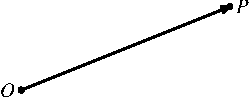
\includegraphics{images/v-1}
\end{center}
\caption{Vektor zwischen zwei Punkten $O$ und $P$, Ortsvektor des Punktes $P$
\label{image-vektor}}
\end{figure}
Ein Punkt $P$ wird durch die Länge der Projektionen der Strecke $OP$
auf die Achsrichtungen festgelegt, also durch ein Zahlenpaar $(x,y)$.
Der Punkt $(1,0)$ liegt auf der $x$-Achse, eine Einheit vom Punkt $O$
entfernt.
Der Punkt $(0,1)$ liegt gleich weit entfernt von $O$ auf der $y$-Achse.

\subsubsection{Ortsvektoren}
Die Einführung eines Koordinatensystems ermöglicht zwar, Punktmengen
in der Ebene durch algebraische Beziehungen zwischen den Koordinaten
zu beschreiben, zum Beispiel ist der Einheitskreis die Menge der
Punkte
\[
\{(x,y)\;|\;x^2+y^2=1\}.
\]
``Rechnen'' kann man mit den Punkten aber noch nicht.
Dazu bilden wir
die Spaltenvektoren, mit denen wir ja bereits zu rechnen gelernt haben,
wie folgt auf die Punkte der Ebene ab:
\[
\begin{pmatrix}x\\y\end{pmatrix}
\mapsto (x,y)
\]
Den Vektor $\begin{pmatrix}x\\y\end{pmatrix}$ können wir uns als
Vektor vom Nullpunkt des Koordinatensystems zum Punkt $P=(x,y)$ vorstellen:
\[
\begin{pmatrix}x\\y\end{pmatrix}
=
\overrightarrow{OP}.
\]
\index{Ortsvektor}
$\overrightarrow{OP}$ heisst
heisst {\em Ortsvektor} des Punktes $P$.
Analoges gilt in drei Dimensionen:
\[
\begin{pmatrix}x\\y\\z\end{pmatrix}
\mapsto
(x,y,z)
\]
Ja es gibt überhaupt keinen Grund, die Geometrie auf zwei oder drei
Dimensionen zu beschränken, wir können Vektoren beliebiger Dimension
auf Punkte
abbilden, die entsprechend viele Koordinaten haben:
\[
\begin{pmatrix}
x_1\\x_2\\\vdots\\x_n
\end{pmatrix}
\mapsto
(x_1,x_2,\dots,x_n)
\]

\subsubsection{Vektoroperationen}
Die Rechenoperationen mit Vektoren können wir ebenfalls in geometrische
Begriffe übersetzen:
\begin{figure}
\begin{center}
\begin{tabular}{cc}
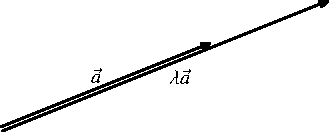
\includegraphics{images/v-2}&
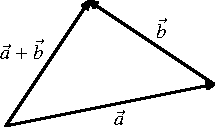
\includegraphics{images/v-3}
\end{tabular}
\end{center}
\caption{Algebraische Operationen mit Vektoren\label{image-vektor-operationen}}
\end{figure}
\begin{itemize}
\index{Streckung}
\item Die Multiplikation mit einer Zahl $\lambda$ ist eine Streckung mit
Zentrum $O$ und Streckfaktor $\lambda$.
\index{Aneinandersetzen}
\item Die Addition von zwei Vektoren entspricht dem ``Aneinandersetzen''
der Strecken.
\end{itemize}
\begin{figure}
\centering
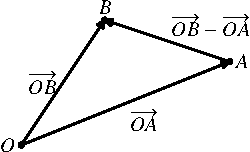
\includegraphics{images/v-4}
\caption{Vektor
%$\overrightarrow{AB}$
\label{image-vektorab}
}
\end{figure}
Besonders im Falle der Addition spielt die ``Richtung'' der Strecken eine
Rolle, wir symbolisieren diese Richtung durch einen Pfeil.
Der Pfeil vom Punkt $A$ zum Punkt $B$ ist die Differenz der Vektoren die von
$O$ zum Punkt $B$ bzw.~zu $A$ führen:
\[
\overrightarrow{AB}=\overrightarrow{OB}-\overrightarrow{OA}
\]

\subsubsection{Vektoren als Translationen}
Vektoren können auch als Verschiebungs-Operationen  oder Translationen
des Raumes betrachtet werden.
Wenn eine Verschiebung den Punkt $A$ in den Punkt $B$ verschiebt,
verschiebt sie den Punkt $C$ in den Punkt $D$ mit Ortsvektor
\[
\overrightarrow{OD}
=
\overrightarrow{OC}+\overrightarrow{AB}
=
\overrightarrow{OC}+\overrightarrow{OB}-\overrightarrow{OA}.
\]
Die Verschiebung entspricht also der Addition eines Verschiebungsvektors
zu allen Ortsvektoren.

\subsubsection{Bemerkungen zur Notation}
In diesem geometrischen Zusammenhang werden wir oft Vektoren als
kleine Buchstaben mit einem Pfeil schreiben: $\vec v$.
Um jedoch interessante
Geometrie zu treiben, müssen wir die üblichen geometrischen Begriffe in
Vektorschreibweise übersetzen: Geraden, Ebenen, Kreise, Kugeln.
Ausserdem müssen wir lernen, wie übliche geometrische Konstruktionen in
Rechenoperationen mit Vektoren übersetzt werden können.

\subsection{Basis}
\index{Basis}
\begin{figure}
\begin{center}
%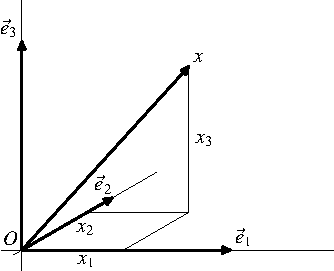
\includegraphics{images/v-5}
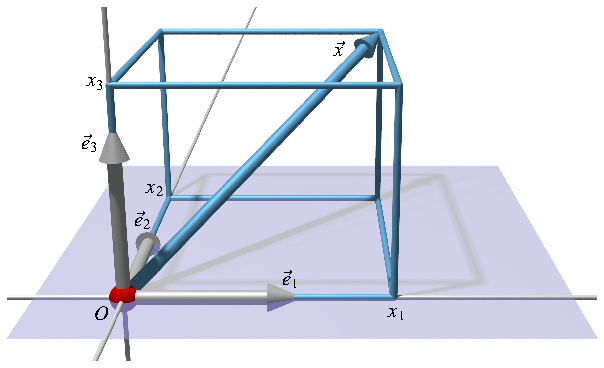
\includegraphics{3/images/coordsystem.pdf}
\end{center}
\caption{Darstellung des Vektors $\vec{x}$ in der Basis
$\{\vec{e}_1,\vec{e}_2,\vec{e}_3\}$ als
$\vec{x} =
x_1\vec{e}_1+
x_2\vec{e}_2+
x_3\vec{e}_3$.
\label{imagebasis}}
\end{figure}
Im Abschnitt \ref{speziellevektoren} haben wir die Vektoren $e_i$
kennengelernt.
Im aktuellen Zusammenhang schreiben wir dafür oft auch
\[
\vec e_1=\begin{pmatrix}1\\0\\0\end{pmatrix},\qquad
\vec e_2=\begin{pmatrix}0\\1\\0\end{pmatrix},\qquad
\vec e_3=\begin{pmatrix}0\\0\\1\end{pmatrix}.
\]
Diese Vektoren konnten dafür verwendet werden, einen beliebigen Vektor
mit Hilfe einer Linearkombination zusammenzusetzen:
\[
\vec v=
v_1\vec e_1+
v_2\vec e_2+
v_3\vec e_3.
\]
Die speziellen Vektoren $e_1,\dots,e_n$ sind nicht die einzig möglichen,
mit denen man die Position eines Punktes auf vektorielle Weise
beschreiben könnte.
Jeder andere Satz von $n$ Vektoren kann
dazu verwendet werden, sofern sich damit jeder beliebige Vektor
linear kombinieren lässt.
In Kapitel~1 haben wir gelernt, dass dies
gleichbedeutend damit ist, dass die Vektoren linear unabhängig sein
müssen.
\begin{definition}
$n$ linear unabhängige Vektoren $b_1,\dots,b_n$ heissen eine
Basis des $n$-dimensionalen Raumes.
\end{definition}
Um die Koordinaten eines Punktes $x$ in dieser Basis zu bestimmen,
müssen die Zahlen $\xi_1,\dots,\xi_n$ berechnet werden für die
gilt
\[
b_1\xi_1+\dots+b_n\xi_n=x.
\]
Ausgeschrieben ist dies das Gleichungssystem
\[
\begin{linsys}{3}
b_{11}\xi_1&+&\dots &+&b_{1n}\xi_n&=&x_1\\
\vdots   & &\ddots& &\vdots&&\vdots\\
b_{n1}\xi_1&+&\dots &+&b_{nn}\xi_n&=&x_n\\
\end{linsys}
\]
Sind die Vektoren linear unabhängig, dann ist die Koeffizientenmatrix
regulär, das Gleichungssystem hat also genau eine Lösung.
Die behauptete Darstellung ist also immer möglich.

Somit haben wir eine weitere Interpretation einer regulären Matrix:
die Spalten einer regulären Matrix sind Vektoren, die man dazu verwenden
kann, jeden beliebigen anderen Vektor linear zu kombinieren.

\begin{beispiel}
Man stelle den Vektor $\vec v$ in der Basis $b_1,b_2,b_3$ dar:
\[
\vec b_1=\begin{pmatrix}2\\-3\\-2\end{pmatrix},\quad
\vec b_2=\begin{pmatrix}6\\-2\\-3\end{pmatrix},\quad
\vec b_3=\begin{pmatrix}-1\\2\\1\end{pmatrix},\qquad
\vec v=\begin{pmatrix}-6\\3\\3\end{pmatrix}.
\]

\smallskip

{\parindent 0pt
Die} Koordinaten $(\xi_1,\xi_2,\xi_3)$ müssen gefunden
werden, so dass
\[
\xi_1\vec b_1+
\xi_2\vec b_2+
\xi_3\vec b_3
=
\vec v,
\]
d.~h.
\[
\xi_1\begin{pmatrix}2\\-3\\-2\end{pmatrix}+
\xi_2\begin{pmatrix}6\\-2\\-3\end{pmatrix}+
\xi_3\begin{pmatrix}-1\\2\\1\end{pmatrix}=
\begin{pmatrix}-6\\3\\3\end{pmatrix}
\quad
\Leftrightarrow
\quad
\begin{pmatrix}
2&6&-1\\
-3&-2&2\\
-2&-3&1
\end{pmatrix}
\begin{pmatrix}\xi_1\\\xi_2\\\xi_3\end{pmatrix}
=
\begin{pmatrix}-6\\3\\3\end{pmatrix}.
\]
Auflösung des Gleichungssystems mit dem Gauss-Algorithmus oder mit
dem Computer ergibt.
\[
\begin{pmatrix}\xi_1\\\xi_2\\\xi_3\end{pmatrix}
=
\begin{pmatrix}1\\-1\\2 \end{pmatrix}.
\]
\end{beispiel}

